\documentclass[CS4204-Notes.tex]{subfiles}
\begin{document}

\section{Haskell implementation}

\subsection{Synchronisation}
Most information is local to a Haskell Execution Context (HEC) and normally HECs do not need to communication except during synchronisation. Synchronisation is needed when
\begin{itemize}
\item Garbage collection is needed
\item A thread becomes blocked on another thread (black hole)
\item When a HEC updates a result that a thread on another HEC is blocked on
\item When exceptions are thrown to another HEC
\item When performing foreign function calls
\item When load balancing happens
\end{itemize}
Most synchronisation is needed when values have to be shared across threads. The GHC creates black holes during garbage collection for each shared closure on the stack, though this is done lazily. Threads then block when they encounter a block hole.\n
Each HEC has its own allocation area which comprises of a number of memory blocks. The garbage collector is invoked when the area becomes full and then proceeds in parallel with the normal execution. This is needed to ensure that one HEC does not write over another HEC's heap. During garbage collection, HECs share information about shared heap objects such as results in data replication. Mutable objects are locked at this stage.

\subsection{Improving granularity}

\subsubsection{Chunking}
Chunking involves grouping multiple data items together before passing it as work to a thread. This increases granularity by allowing a single task to deal with more work and help reduce thread creation overhead.
\begin{figure}[H]
  \centering
  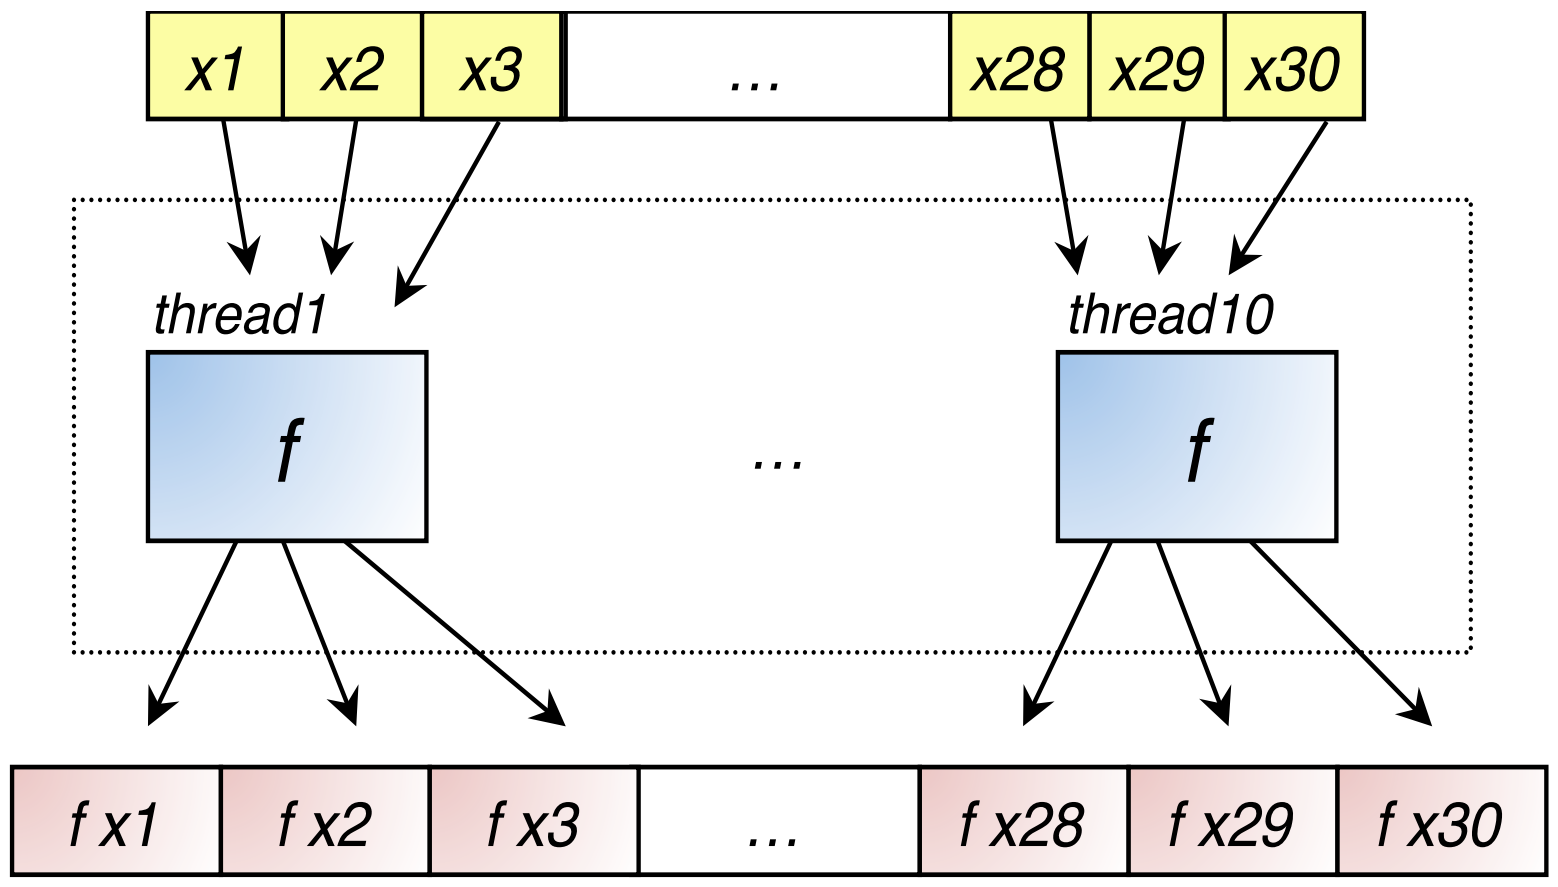
\includegraphics[width=0.6\textwidth, keepaspectratio]{imgs/chunking.png}
\end{figure}

\subsubsection{Buffering}
Buffering can be done to ensure threads are not flooded with work. In this approach, only the first few threads are passed data to work on and the rest are created as the threads complete. 


\subsection{Tuning for multicore}
There are four main issues in tuning parallel code for multicore architectures:
\begin{enumerate}
\item Good granularity
\item Cache/memory locality
\item Minimising locking costs
\item Limiting thread creation overheads
\end{enumerate}

\subsubsection{Core affinity}
Core affinity is the concept of keeping the same threads on the same core. This is done for reasons of cache and power usage. By keeping the threads on the same core, data may be still kept in the cache, which allows for better usage. Furthermore, for power usage reasons it may be better to maintain similar usage levels on all cores.
The following flags in GHC allow a programmer to define the affinity
\begin{itemize}
\item \texttt{ghc -qa}, use the OS to set affinity for worker tasks
\item \texttt{ghc -qm}, don't automatically migrate worker tasks between cores
\item \texttt{ghc -qw}, migrate to the current core when a worker task is woken
\end{itemize}

\subsubsection{Virtual cores}
In some modern CPUs, a single real core is split into two or more virtual cores. This gives the illusion of having more cores, allowing idle units to do more work, but with simulaneous multithreading. Using virtual cores has many disadvantages compared to real cores:
\begin{itemize}
\item Real cores don't share a memory pipeline - This means there will be fewer cache misses as real cores will have separate caches. This leads to a smaller chance of threads stalling due to writing back changed data
\item Real cores have more real hardware units - more intensive code can use all available units, so having two virtual cores on one real core would create conflict over resource usage
\item Simultaneous multithreading can be much slower than multi-core due to cache thrashing
\end{itemize}

\end{document}